\part{Mass-Spring Systems}
\begin{multicols}{2}
Steps towards a simulation of a Mass-Spring system:
\begin{itemize}
\item \emph{Spatial discretization}: Sample object with mass points
\item \emph{Forces}: Define internal (springs!) and external forces
\item \emph{Dynamics}: Set up equations of motion
\item \emph{Temporal discretization}: Solve equations of motion
\end{itemize}

\section{Spatial Discretization}
    Sample object with mass points:
    \begin{align*}
    	\text{Total mass of object: }& M,\\
    	\text{Number of mass points: }& n,\\
    	\text{Mass of each point: }& m = {M \over n},
    \end{align*}
    with each point holding the properties:
    \begin{align*}
    	\text{Mass: }&m_i\\
    	\text{Position: }& x_i(t)\\
    	\text{Velocity: }& v_i(t) 
    \end{align*}

\section{Forces}
 What are the forces that act on particle $i$?
	\begin{description}
		\item[External Forces] Gravity: $F_i$
		\item[Internal Forces] $\textbf{}$
			\begin{itemize}
				\item Elastic spring forces
				\item Viscous damping forces
			\end{itemize}
		\item[Total force] $F_i = F_i^{int} + F_i^{ext}$
	\end{description}

\subsection{Internal Forces}
\subsubsection{Elastic Springs}
\begin{definition}[Elasticity]
	Ability of a spring to return to its initial length when the deforming force is removed. 
\end{definition}

\begin{align*}
	F & =-k(l-L) & \text{Hooke's Law } (1D)\\
	F_i &= -k(||\vec x_i - \vec x_j || - L) {\vec x_i - \vec x_j \over ||\vec x_i - \vec x_j || } & (3D)\\
	L: &\quad \text{ Initial spring length}\\
	l: &\quad \text{ Current spring length}\\
	k: &\quad \text{ Spring stiffness}
\end{align*}
For purely elastic springs \emph{the force depends only on the position} and \emph{no energy is lost during the deformation}.
\begin{align*}
	W &=\int_L^l k(x-L) dx &\text{Work done by forces}\\
	E &= W= {1 \over 2} k(l-L)^2 &\text{Elastic spring energy}\\
	\vec F_i &= -{\del E \over \delta \vec x_i} &\text{Force}
\end{align*}

\paragraph{Forces at Mass Point} internal forces $F_0^{int}$:
\begin{align*}
	\vec F_0^{int} &= -\sum_{i|i\in \{1,2,3\}} k_i (l_i-L_i) {\vec x_i - \vec x_0 \over l_i}
\end{align*}
\begin{figure}[H]
	\centering
	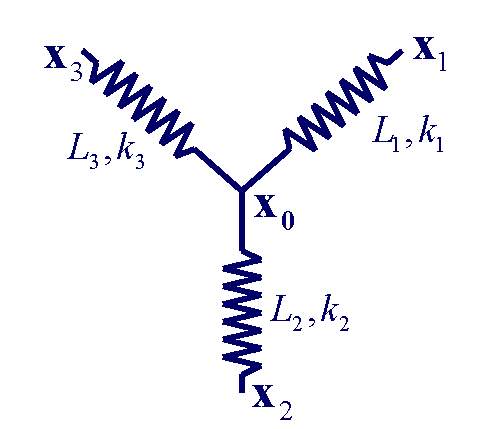
\includegraphics[width=0.4\textwidth]{img/01_forces_at_mass_point.pdf}
	\caption{Example}
\end{figure}

\subsection{Dissipative Forces}
Real-world mechanical systems dissipate energy over time: \emph{Internal friction $\implies$  Thermal energy} (irreversible process). Controllable dissipation is useful for physics simulations. 
\paragraph{Dissipation for mass-spring systems} $\gamma$ is the damping coefficient
\begin{align*}
\vec F^{pd} (t) &= -\gamma\cdot \vec v(t) &\text{Point damping}
\end{align*}
Point damping is simple and efficient, but it \emph{damps \textbf{all} motion} (i.e. including translations and rotations).

\subsection{External Forces}
External forces are forces like
\begin{itemize}
	\item Gravity
	\item Contact forces
	\item All forces that are not cause by springs
\end{itemize}

\section{Dynamics}
In the dynamics step the equations of motion are setup. The force is known for every particle.
    \paragraph{Kinematic relations}
		\begin{align*}
			\textbf{Velocity: }\vec v_i(t) &= {d \vec x_i (t) \over dt}\\
			\textbf{Acceleration: }\vec a_i(t) &= {d\vec v_i(t) \over dt} = {d^2 \vec x_i(t) \over dt^2}
		\end{align*}

With \textbf{Newton's $2^\text{nd}$ Law} 
\begin{align*}
\vec F_i &=m_i \cdot \vec a_i
\end{align*}
we can describe the equations of motion using Newton's second law:
\begin{align*}
	\vec F_i &= m_i {d^2 \vec x_i (t) \over d t^2} = \vec F_i^{int}(t) + \vec F_i^{ext}(t)\\
	&\text{which can be abstracted as}\\
	\vec F  &= M {d^2 \vec x (t) \over d t^2} = \vec F^{int}(t) + \vec F^{ext}(t) & M \in \R^{3n\times 3n}\\
	&\text{adding damping}\\
&	M {d^2 \vec x (t) \over d t^2} + D {d\vec x(t) \over dt}= \vec F^{int}(t) + \vec F^{ext}(t)
\end{align*}

\section{Temporal discretization}
A \emph{differential equation} describes an unknown function through its derivatives. An ordinary differential equation (ODE) contains only derivatives with respect to a single variable.

\begin{tabular}{c|c}
	\textbf{Example}&\textbf{Abstract form}\\ \hline
	$x''(t) = {\vec F(t) - \gamma \vec x'(t) \over m_i}$&
	$y''(t) = f(t, y, y')$
\end{tabular}
The order of the ODE is expressed as function of the highest derivative:
\begin{align*}
	y^{(n)} = f(x, y, y',y'',\ldots,y^{(n-1)}).
\end{align*}

Solving an ODE: Given $f$, determine $y$. Example:
\[
	y'(t) = f(t,y) = y(t) \quad \Longrightarrow\quad y(t) = Ce^t
\]
The integration constant $C$ is unknown and i determined by the initial value:
\begin{align*}
	y(0) =2 \qquad \Longrightarrow \qquad C = 2
\end{align*}
\emph{ODE + initial value = initial value problem (IVP)}

\begin{theorem}{Picard–Lindelöf}
An IVP has a unique solution if $f$ is Lipschitz continuous.
\end{theorem}
\subsection{Application to Mass-Spring systems}
We have an initial position $\vec x_i(t_0)$, an initial velocity $\vec v_i (t_0)$ and a governing ODE:
\begin{align*}
	{d^2 \vec x_i (t) \over dt^2} = {\vec F_i(t) - \gamma \vec v_i(t) \over m_i}.
\end{align*}
We want the position $\vec x_i$ over time. 

The first step to rewrite the problem since it's easier to deal with as a first oder ODE. We therefore reduce the $2^{nd}$ order ODE to two coupled $1^{st}$ order ODEs.
\begin{align*}
	&m_i {d^2 \vec x_i(t) \over dt^2} + \gamma {d \vec x_i (t) \over dt} = \vec F_i (t) \\
	&\begin{cases}
		{d \vec x_i(t) \over dt} = \vec v_i (t) & \text{velocity} \\
		{d \vec v_i(t) \over dt} = {\vec F_i (t) - \gamma \vec v_i (t) \over m_i} & \text{acceleration}
	\end{cases}
\end{align*}

Write as one system of $1^{st}$ order ODEs:
\begin{align*}
	\vec y_i (t) &= \begin{pmatrix}
 						\vec x_i(t)\\
 						\vec v_i(t)
 					\end{pmatrix}\\
	\vec y_i' (t) &=  \begin{pmatrix}
  						\vec v_i(t)\\
  						{\vec F_i (t) - \gamma \vec v_i (t) \over m_i}
  					   \end{pmatrix}
\end{align*}

\subsection{Numerical Solution}
Compute approximations $y_i$ to true solution for \emph{discrete} time instants $t_i$. Compute solution at $t_{i+1}$ based on previous solutions at $t_{i-1}$, $t_{i-2}$.
\begin{figure}[H]
	\centering
	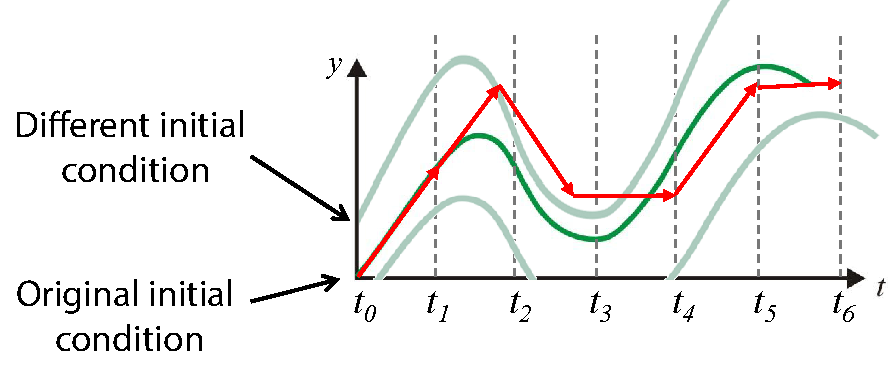
\includegraphics[width=0.45\textwidth]{img/01_initial_conditions}
	\caption{Solutions based on different initial conditions}
\end{figure}

\section{Integration schemes} $\textbf{}$
\begin{description}
	\item[Explicit Methods] $\textbf{}$
		\begin{itemize}
			\item Explicit Euler
			\item Heun, Midpoint
			\item Runge-Kutta methods
		\end{itemize}
		Tend to explode with \emph{stiff problems}:
		\begin{itemize}
			\item Explicit methods require very small time steps for stable integration
			\item Are inefficient since step size is determined by stability not accuracy requirements. 
		\end{itemize}
		Use implicit methods for stiff problems.
	\item[Implicit Methods] $\textbf{}$
		\begin{itemize}
			\item Backward Euler
			\item Implicit Euler
			\item BDF methods
		\end{itemize}
	\item[Methods for higher order ODEs] $\textbf{}$
		\begin{itemize}
			\item Verlet
			\item Leapfrog
			\item Newmark methods
		\end{itemize}
\end{description}

\subsection{Computing Approximations} An approximation of a function $y(t)$ can be computed by computing the taylor expansion:
\begin{align*}
	y(t+h) &= y(t) + {y'(t) \over 1!}h + {y''(t) \over 2!}h^2 + \ldots,
\end{align*}
which allows us to compute a first order approximation:
\begin{align*}
	y(t+h) &= y(t) + hy'(t).
\end{align*}
Which leaves us with \emph{Euler' Method}.

\subsubsection{Accuracy criteria} to evaluate an integration scheme:
\begin{description}
	\item[Convergence] Do approximations converge to true solution, i.e. 
		\[
			h\mapsto 0 \implies y_i \mapsto y_i(t)
		\]
	\item[Accuracy] how fast does the error decrease as $h\mapsto 0$\\
		Local error is $\bigO{h^{p+1}}$ $\implies$ Method is accurate of order $\mathbf p$.
	\item[Stability] Is the solution always bounded, i.e. $|y_n| < \infty$
	\item[Efficiency] Is a given method a good choice for a given problem?
\end{description}

\subsubsection{Euler's Method} Start at the initial condition and take a step into the direction of the tangent.
\begin{align*}
	y_{n+1} &= y_n + hf(t_n, y_n).
\end{align*}

\begin{figure}[H]
	\centering
	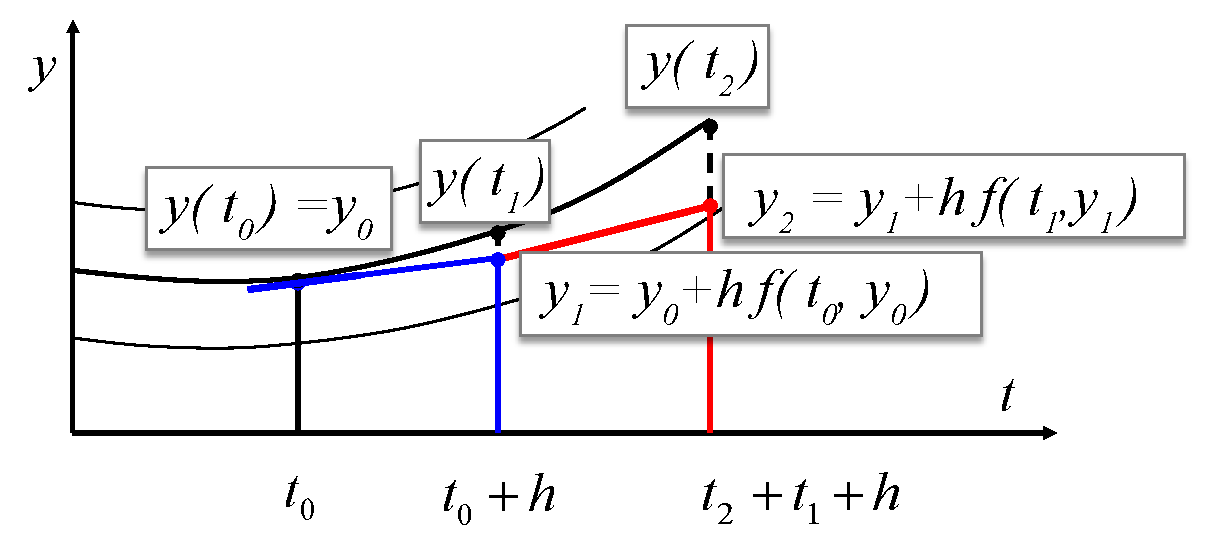
\includegraphics[width=0.45\textwidth]{img/01_euler}
	\caption{Visualization of the Euler Method}
\end{figure}

Explicit Euler has an accuracy of order $1$: $\bigO{h^2}$ error per stop.


\subsubsection{Heun's Method}
Heun's method is a two step method and provides a $\mathbf{2^{nd}}$ \textbf{order accuracy}. Idea:
\[
	y(t+h) \approx y(t) + {h \over 2} [y'(t) + y'(t+h)],
\]
$y'(t+h)$ is unknown. Use an Euler step to compute it. 
\begin{align*}
	\tilde y_{n+1} &= y_n + h\cdot f(t_n, y_n) \\
	y_{n+1} &= y_n + {h \over 2} \left[ f(t_n, y_n) + f(t_{n+1}, \tilde y_{n+1}) \right]
\end{align*}

\begin{figure}[H]
	\centering
	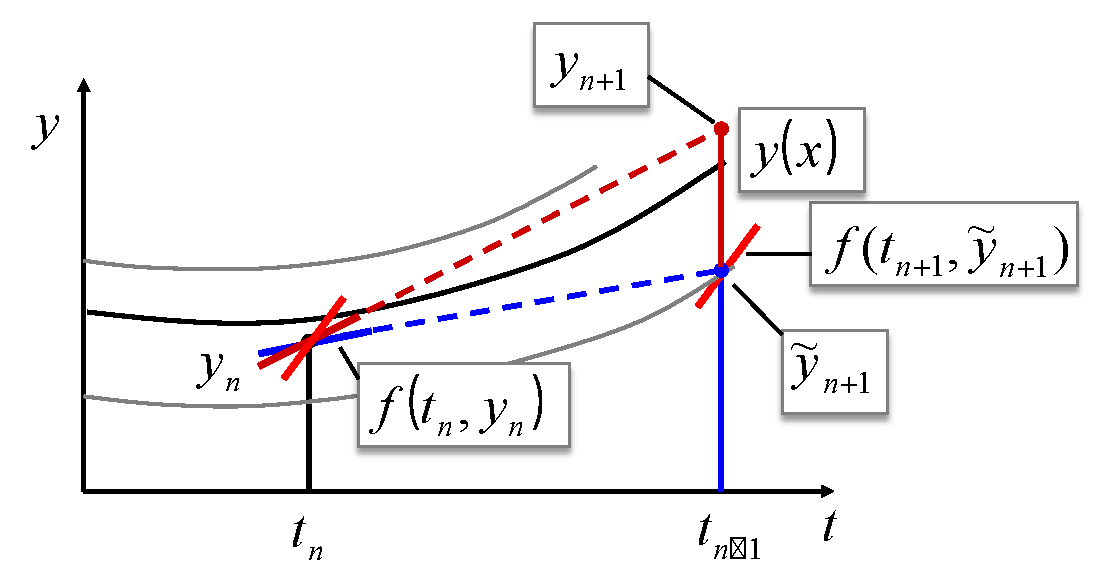
\includegraphics[width=0.45\textwidth]{img/01_heun}
	\caption{Heun's Method graphically}
\end{figure}

\subsubsection{Explicit Midpoint Method}
Heun's method uses $f(t)$ and $f(t+h)$ to achieve $2^{nd}$ order accuracy. Use $f\left(t+{h\over 2} \right)$ instead. This also gives us $2^{nd}$ order accuracy.

\begin{align*}
	\tilde y_{n+1} &= y_n + {h \over 2}\cdot f(t_n, y_n) \\
	y_{n+1} &= y_n + h \left[ f(t_n, y_n) + f(t_{n+1}, \tilde y_{n+1}) \right]
\end{align*}
This solution provides us also with provides a $\mathbf{2^{nd}}$ \textbf{order accuracy}.

\subsubsection{$\mathbf{4^{th}}$-Order Runge-Kutta}
\emph{RK4} is one of the most widely used integrators. Four slope evaluations gives us $\mathbf{4^{th}}$ \textbf{order accuracy}
\begin{align*}
	k_1 &= f\left(t_n, y_n\right)\\
	k_2 &= f\left(t_n+{1\over 2}h, y_n+{1\over 2}k_1\right)\\
	k_3 &= f\left(t_n+{1\over 2}h, y_n+{1\over 2}k_2\right)\\
	k_4 &= f\left(t_n+h, y_n + h k_3\right)
\end{align*}
$y_{n+1}$ is computed using a weighted average slope:
\begin{align*}
	y_{n+1} &= y_n + {1 \over 6}h (k_1 + 2k_2 + 2k_3+k_4)
\end{align*}
\begin{figure}[H]
	\centering
	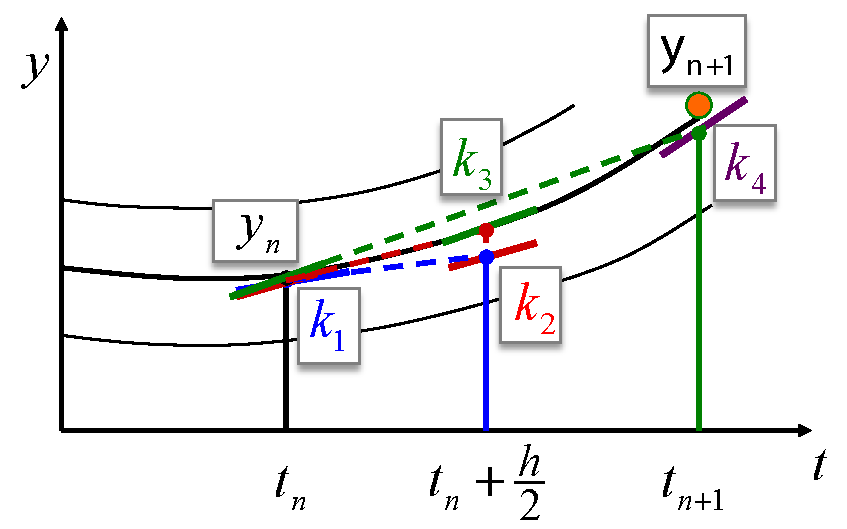
\includegraphics[width=0.45\textwidth]{img/01_rk4}
	\caption{RK4 graphically}
\end{figure}


\end{multicols}
